React (иногда React.js или ReactJS) — JavaScript-фреймворк с открытым исходным кодом для разработки пользовательских интерфейсов.

React разрабатывается и поддерживается Facebook, Instagram и сообществом отдельных разработчиков и корпораций.

React может использоваться для разработки одностраничных и мобильных приложений. Его цель — предоставить высокую скорость,
простоту и масштабируемость. В качетсве библиотеки для разработки пользовательских интерфейсов, React часто используется с другими библиотеками,
такими как Redux.

React был создан Джорданом Уокером, разработчиком програмного обеспечения из Facebook. На него оказал влияние XHP — компонентный HTML фреймворк для PHP.
В первый раз React был использован в новостной ленте Facebook в 2011 году и позже в ленте Instagram в 2012 году. Исходный код React был открыт в мае 2013
года на конференции «JSConf US».

React Native был анонсирован на конференции Facebook «React.js Con» в феврале 2015 года, а исходный код был открыт в марте 2015 года. Он позволяет
разрабатывать нативные Android, iOS и UWP приложения с использованием React.

18 апреля 2017 года Facebook анонсировал React Fiber, переписанную и оптимизированную версию React. React Fiber станет основой разработки всех
будущих функций и улучшений.

Ниже приведен пример использования React в HTML с JSX и JavaScri-pt.

\begin{lstlisting}[language=HTML, label=lst:domain:reactjs]
<div id="myReactApp"></div>

<script type="text/babel">
  
  class Greeter extends React.Component { 
    
    render() { 
      return <h1>{this.props.greeting}</h1>
    } 

  } 

  ReactDOM.render(
      <Greeter greeting="Hello World!" />,
      document.getElementById('myReactApp')
  );

</script>
\end{lstlisting}

Класс Greeter это React компонент, который принимает свойство gree-ting. Метод ReactDOM.render отрисовывает
экземпляр класса (компонента) Greeter с свойством greeting равным 'Hello World' и вставляет отрисованный компонент в
DOM-элемент с идентификатором myReactApp как вложенный элемент.

При отображении в веб-браузере, результат будет

\begin{lstlisting}[language=HTML, label=lst:domain:html]
<div id="myReactApp">
  <h1>
    Hello World!
  </h1>
</div>
\end{lstlisting}

В контексте данной работы, фреймворк Reactjs можно применить для реализации пользовательского интерфейса приложения-обертки
над компонентами WebGL. Поскольку реализация стандартных механизмов валидации компонентов пользовательского интерфейса может
быть затруднительна, а основная часть работ при реализации любого приложения-редактора -- дизайн и создание пользовательского
интерфейса, целесообразно использовать стандартные возможности HTML/CSS для проектирования пользовательского интерфейса и
использование парадигмы Redux с функциональным подходом к разработке кода для создания системы основанной на централизованном
хранилище состояния.

Для упрощения взаимодействия между компонентами системы предлагается использование парадигмы Redux. Redux -- система для управления
состоянием в приложении. Поддерживает возможность реализации полностью функционального кода, избавляя приложение от необходимости
ручной мутации состояния, преобразуя его в канонический автомат Мили.

Функции переходов такого автомата реализуются с помощью так называемых модулей-Reducer'ов (отсюда и название библиотеки), а состояние
в любой момент времени определяется как применение того или иного Reducer'а к текущему состоянию. Определение подходящей ветки
работы Reducer'а производится исходя из типа действия, выполняемого пользователем в приложении.

Поскольку подобная система является абсолютно чистой с точки зрения мутации данных в приложении, становится возможна реализация
сохранения истории работы пользователя, а так же, ввиду обратимости всех чистых изменений или возможности сохранения истории
<<снимков состояния>> приложения, возможно просто реализовать механизм отката произвольного количества действий пользователя.

На такую систему, однако, накладывается ряд ограничений:

\begin{enumerate}[label=\arabic*.]
\item Все изменения должны быть строго детерменированы, то есть не допускается использование модуля Random.
\item В системе должен быть один источник состояния, называемый Data Store
\item Все промежуточное состояние приложения должно следовать по пути от высокоуровневого компонента иерархии к низкоуровневым.
\end{enumerate}

\begin{figure}[ht]
\centering
  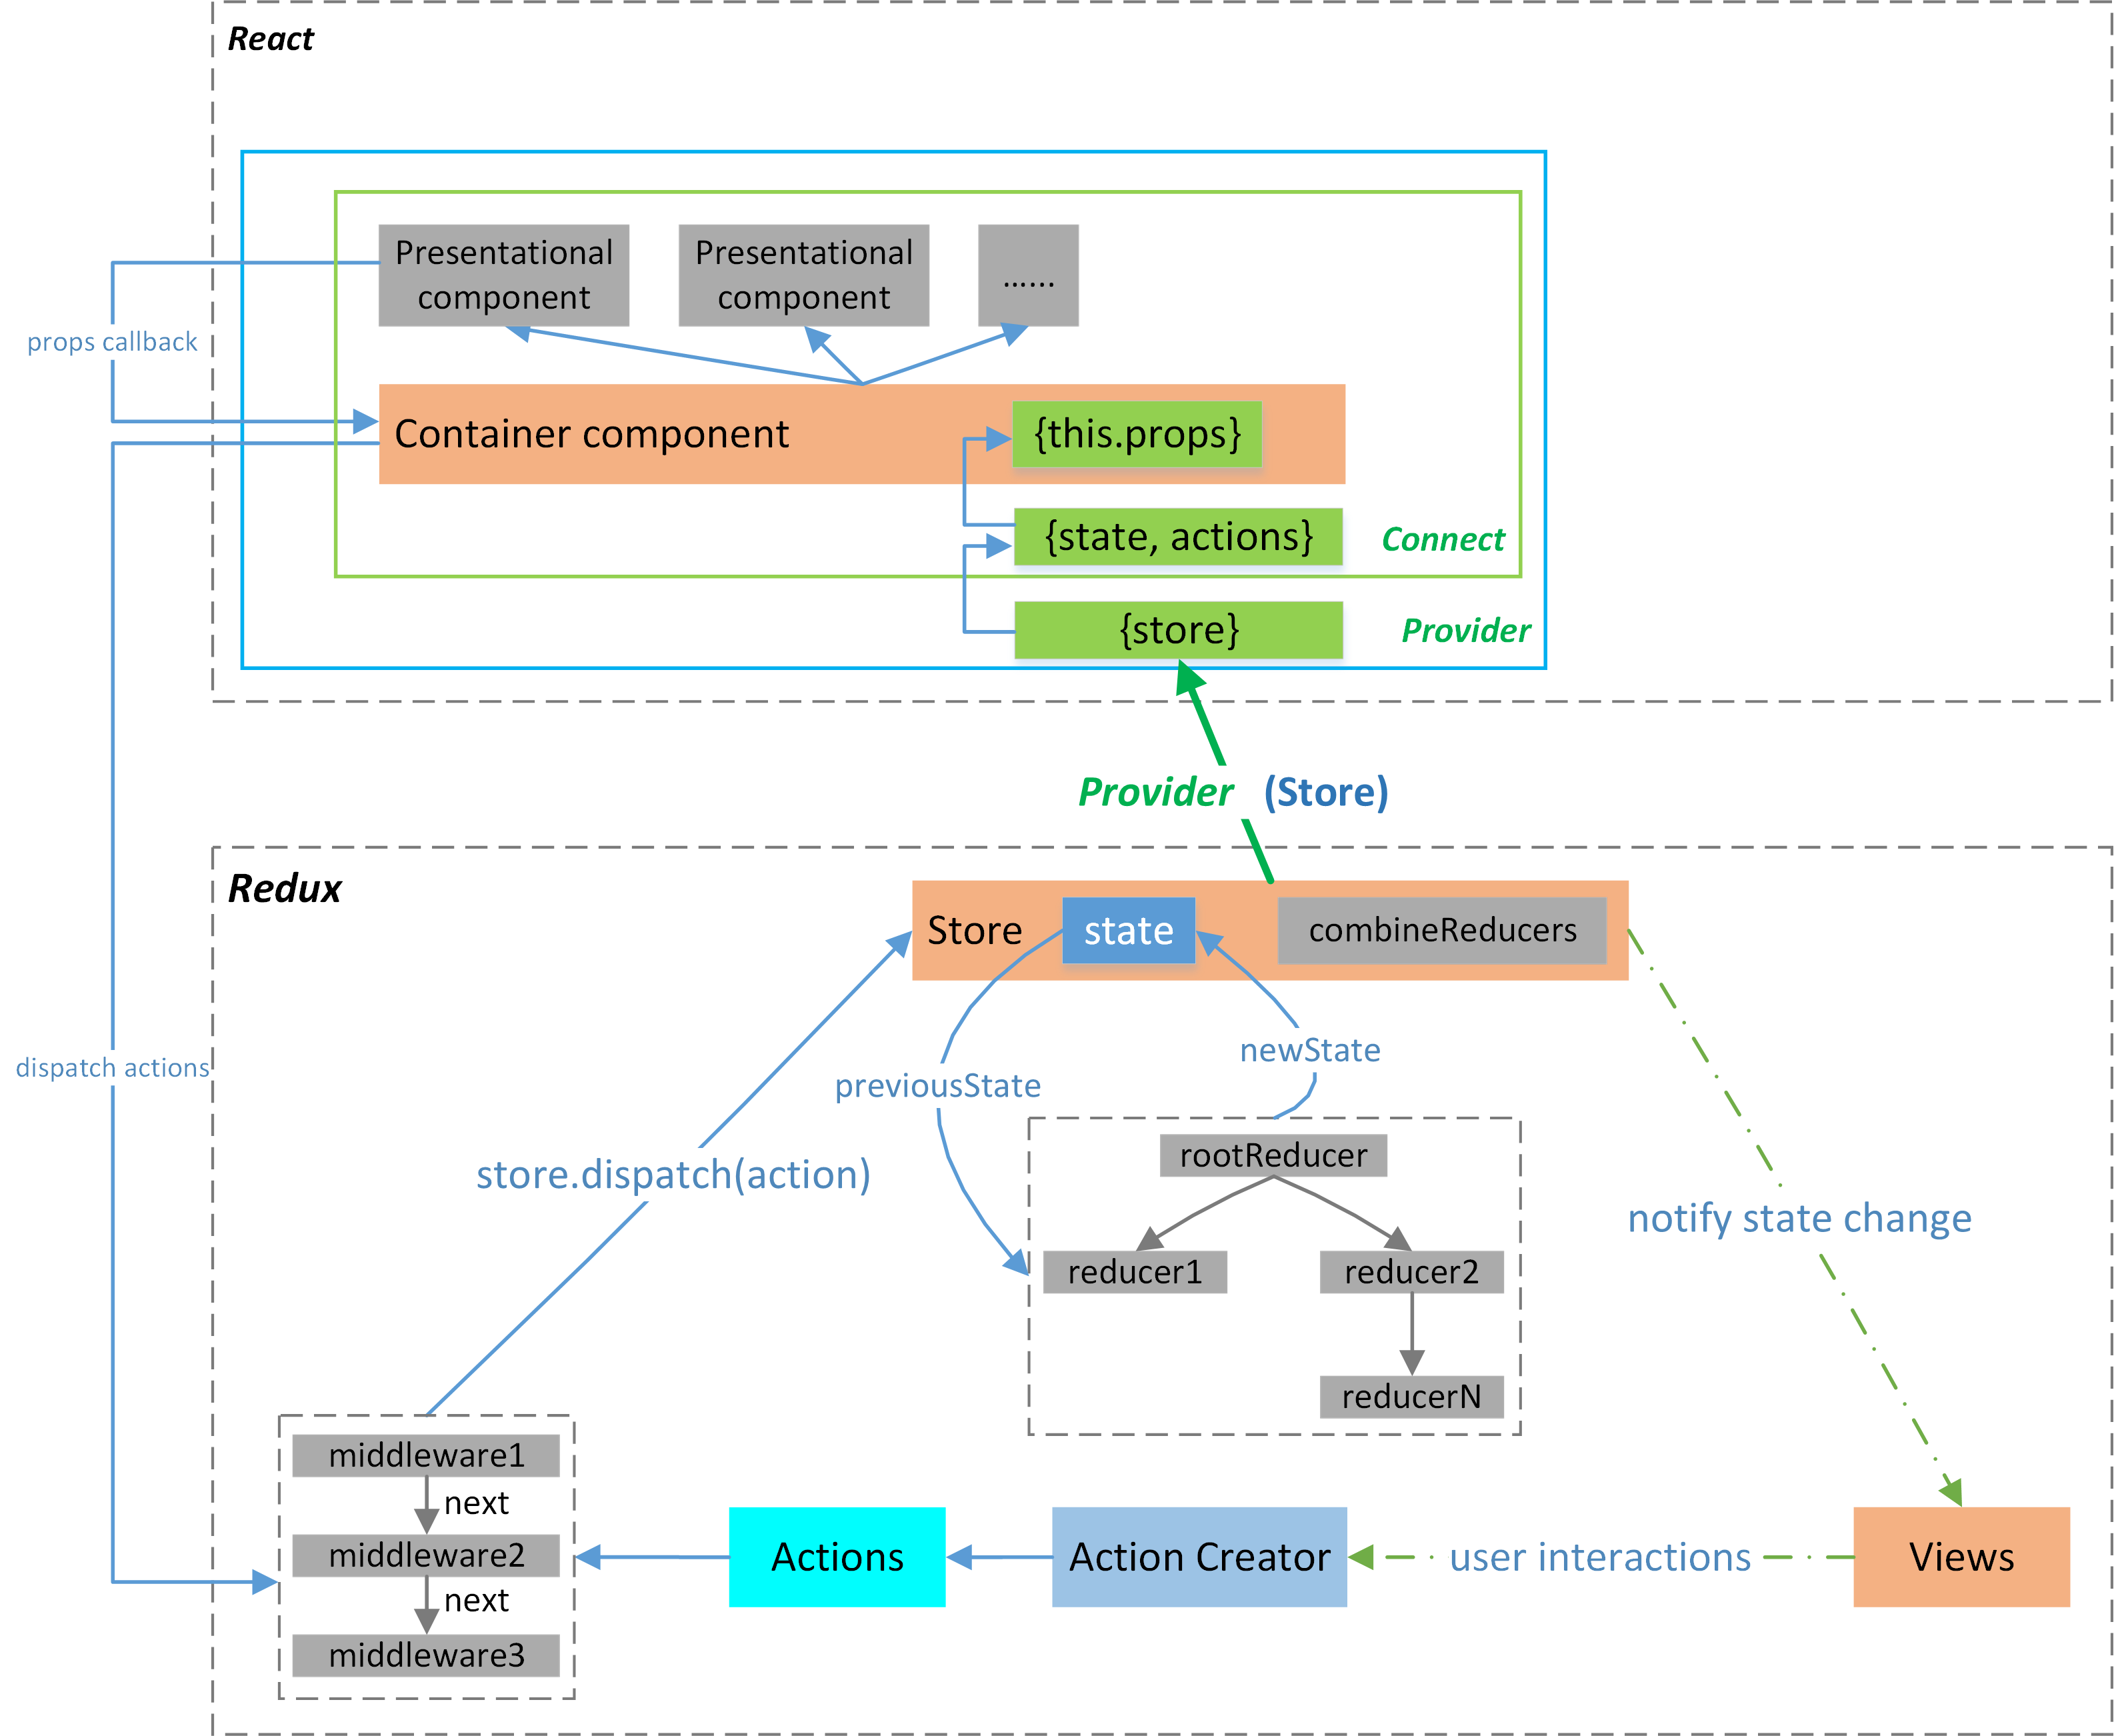
\includegraphics[scale=0.80]{react_redux.png}
  \caption{Диаграмма взаимодействия компонентов в React-Redux приложении}
  \label{figure:domain:react_redux}
\end{figure}

Жизненный цикл Redux-приложения заключается в следующих четырех шагах:

\begin{enumerate}[label=\arabic*.]
\item
 Вызов метода store.dispatch(action)
 Аргумент action содержит метаинформацию о типе действия, произведенного пользователем. Действия могут быть описаны следующими JSON-объектами:
 \begin{lstlisting}[language=TypeScript, label=lst:domain:redux0]
 {
  type: 'LIKE_ARTICLE',
   articleId: 42
 }

 {
   type: 'FETCH_USER_SUCCESS',
   response: {
     id: 3,
     name: 'Mary'
   }
 }

 {
   type: 'ADD_TODO',
   text: 'Read the Redux docs.'
 }
 \end{lstlisting}
 Действия могут быть иницированны из любой точки приложения, имеющий доступ к центральному хранилищу состояния, включая всевозможные компоненты, события XHR, запланированные интервалы.

\item
  Вызов reduce-метода хранилищем состояния. Reduce-метод имеет следующую сигнатуру:
  \begin{lstlisting}[language=TypeScript, label=lst:domain:redux1]
    (Si, Ai) => Si+1
  \end{lstlisting}

  Примером типичного reduce-метода может служить следующий метод из классического 

  \begin{lstlisting}[language=TypeScript, label=lst:domain:redux2]
  let previousState = {
    visibleTodoFilter: 'SHOW_ALL',
    todos: [
      {
        text: 'Read the docs.',
        complete: false
      }
    ]
  }

  let action = {
    type: 'ADD_TODO',
    text: 'Understand the flow.'
  }

  let nextState = todoApp(previousState, action)

  \end{lstlisting}

  Reducer-метод является чистой функцией, то есть он лишь вычисляет новое состояние. Функция-reducer должна быть абсолютно детерменированной:
  вызое ее с одними и теми же аргументами обязан всегда производить точно такие-же результаты, а так-же не должен сопровождаться побочными эффектами,
  такими как изменение маршрута веб-приложения, вызова сторонних API. Все подобные изменения должны производиться до того как действия вызываются.

\item
  Корневая reduce-функция может комбинировать результаты нескольких дочерних reduce-функций для получения полного состояния системы после произведения пользовательских операций.
  Стандартный метод комбинирования reduce-функций - вспомогательный метод combineReducers(), предоставляемый Redux. Ниже указан пример использования combineRedu-cers:

  \begin{lstlisting}[language=TypeScript, label=lst:domain:redux3] 
  function todos(state = [], action) {
    return nextState;
  }

  function visibleTodoFilter(
    state = 'SHOW_ALL',
    action)
  {
    return nextState;
  }

  let todoApp = combineReducers({
    todos,
    visibleTodoFilter
  });

 \end{lstlisting}

 Таким образом, когда пользователь производит действие, будет вызвана комбинация двух reduce-методов, что,
 однако, не приводит к гонкам из-за отсутствия в них побочных дейстивий:
 
 \begin{lstlisting}[language=TypeScript, label=lst:domain:redux4]
 let nextTodos = todos(state.todos, action)
 let nextVisibleTodoFilter =>
   visibleTodoFilter(state.visibleTodoFilter, action)

 return {
    todos: nextTodos,
    visibleTodoFilter: nextVisibleTodoFilter
  }
 \end{lstlisting}

\item
 Reduce-метод сохраняет состояние системы в хранилище состояния и вызвает перерисовку пользовательского интерфейса посредством вызова всех событий, на которые подписана UI система:

 \begin{lstlisting}[language=TypeScript, label=lst:domain:redux5]
   onComponentDidMount: () => {
     store.subscribe((newState) =>
       component.setState(newState)
     );
   } 
 \end{lstlisting}

\end{enumerate}